\chapter{Mapping BPMN to Jiac AgentBeans}
\label{chap:mapping}
The element mapping from BPMN to Jiac AgentBeans is created based on the existing mapping to JiacV - JADL script. In comparation to a JADL script, an AgentBean is written completely in Java, enabling more possibilities in mapping concepts such as intermediate Event handling. This chapter will provide a detailed overview of the mapping.\\\\

%%%%%%%%%%%%%%%%%%%%%%%%%%%%%%%%%%%%%%%%%%%%%%%%%%%%%%%
% 4.1 Pools & Processes                               %
%%%%%%%%%%%%%%%%%%%%%%%%%%%%%%%%%%%%%%%%%%%%%%%%%%%%%%%
\section{Pools and Processes}
Every pool in a process diagram will be mapped into an AgentBean. The name of the AgentBean will be derived from the Pool name, and the name of the process diagram it is contained in. If a Pool with the same name (e.g Mathematican) is contained in the business process diagrams ExtractRoot and Faculty, then the two agent beans \texttt{Mathematican\_ExtractRoot} and \texttt{Mathematican\_Faculty} will be created. Further, they are grouped in the package mathematican. 

The process contained in a pool is mapped into a \textbf{workflow method}. Depending on the start event's type, this workflow method may be called in the execute method of the bean (for timer start event), it may be exposed as an action (for message start event with service implementation), or if the start event is a message start event with MessageChannel implementation, a SpaceObserver will be created and attached to the agent's memory, which will call the workflow method when a message with the payload and address as specified in the implementing message channel are written into the agent's memory.

The mapping of a task contained in a process flow will be wrapped in the so called \textbf{activity method} which will be called by the workflow method. Special cases for tasks with event handler and subprocesses will be discussed in a later section.

Lanes are currently ignored. A process of a lane will be handled as a process of the containing pool.

\begin{figure}[h]
	\centering
		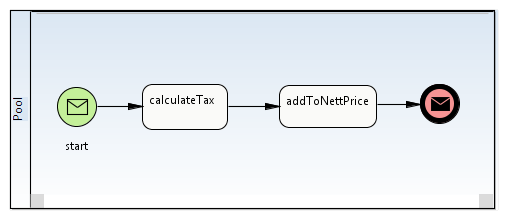
\includegraphics[width=0.80\textwidth]{images/mapping/pool_and_process.png}
	\caption{Mapping example : Pool and Process}
	\label{fig:pool+process}
\end{figure}

The Figure\ref{fig:pool+process} shows a simple example of a pool called Pool with the process doProcess. For the Pool, a Java class called Pool\_DoProcess will be created and it will have the workflow method called doProcess. In this example the message start event is implemented as a service, thus the workflow method is exposed as an Action as we can see in the following Listing \ref{list:pool+process}.  
\begin{lstlisting}[language = Java, caption =  Mapped element: Pool and Process (Figure \ref{fig:pool+process}), label = list:pool+process]
package pool;//derived from the pool name

//some imports...

public class Accounting_CalculatePrice extends AbstractMethodExposingBean{
	
	public final static String ACTION_DOPROCESS = "pool.Pool_DoProcess#doProcess"; 
	
	// process attribute would be declared here
	[...]
	@Expose(name = ACTION_DOPROCESS, scope = ActionScope.GLOBAL)
	public double doProcess(double nettPrice, double taxRateInPercent) {
		calculateTax();
		addToNettPrice();
		return totalPrice;
	}
	
	private void calculateTax(){
		[...]
	}
	
	private void addToNettPrice(){
		[...]
	}
}
\end{lstlisting}


\section{Workflow Structure}
Workflow structure is mapped as the content of the workflow method. It defines the invocation structure of the flow objects contained in a process.

\subsection{Sequence Flow}
The mapping of a sequence flow is trivial. The mapped elements connected with a sequence flow will be invoked sequentially in the workflow method (see Figure \ref{fig:mapping_sequence}).\\

\begin{figure}[h]
	\begin{tabularx}{\linewidth}{lcX}
		\multirow{3}{*}{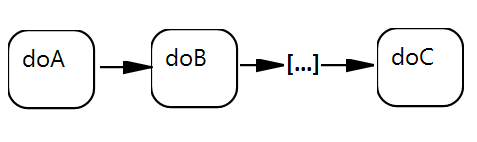
\includegraphics[width=0.4\textwidth]{images/mapping/sequence.png}} &  &	\texttt{	doA();}\\
		& \textbf{\textcolor{blue}{=}}& \texttt{	doB();}\\
		& & \texttt{	doC();}\\
	\end{tabularx}
\caption{Mapping : Sequence Flow}%
\label{fig:mapping_sequence}%
\end{figure}

\subsection{Gateways}
Branches of a gateway are wrapped according to the gateway's type. There are 5 different types of gateways:
\begin{enumerate}
	\item AND (Parallel)
	\item OR (Inclusive)
	\item XOR\_Data (Exclusive)
	\item XOR\_Event (Event Based)
	\item Complex 
\end{enumerate}

%%%%%%%%%%%%%%%%%%%%%%%%%%%%%%%%%%%
\textbf{AND-Gateway (Parallel)}\\
In an AND-Gateway, all branch will be wrapped in parallel to one another. At runtime all branches are executed within a thread. 
Figure \ref{fig:mapping_AND} shows an example of the mapping. \\

\begin{figure}[h]
\begin{tabularx}{\linewidth}{lcX}
	\multirow{18}{*}{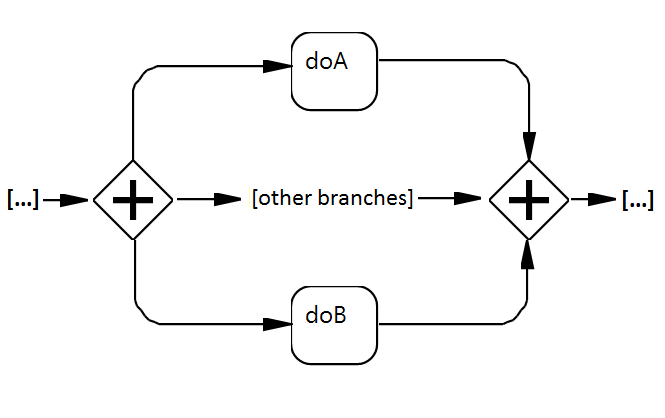
\includegraphics[width=0.3\textwidth]{images/mapping/and-gateway.png}} &  & \texttt{[...]}\\
	& & \texttt{Thread and\_branch1 = new Thread()\{}\\
	& & \texttt{\hspace{10pt}public void run()\{}\\
	& & \texttt{\hspace{20pt}doA();}\\
	& & \texttt{\hspace{10pt}\}}\\
	& & \texttt{\};}\\
	& & \texttt{Thread and\_branch2 = new Thread()\{}\\
	& & \texttt{\hspace{10pt}public void run()\{}\\
	& \textbf{\textcolor{blue}{=}} & \texttt{\hspace{20pt}doB();}\\
	& & \texttt{\hspace{10pt}\}}\\
	& & \texttt{\};}\\
	& & \texttt{and\_branch1.start();}\\
	& & \texttt{and\_branch2.start();}\\
	& & \texttt{try \{}\\
	& & \texttt{\hspace{10pt}and\_branch1.join();}\\
	& & \texttt{\hspace{10pt}and\_branch2.join();}\\
	& & \texttt{\} catch(InterruptedException) \{ \}}\\
	& & \texttt{[...]}\\
\end{tabularx}
\caption{Mapping : AND Gateway}%
\label{fig:mapping_AND}%
\end{figure}

%%%%%%%%%%%%%%%%%%%%%%%%%%%%%%%%%%%%%
\textbf{OR-Gateway (Inclusive)}\\
Branches of an OR-Gateway will also be executed in parallel to one another, but the content of a branch is additionally wrapped in an if-then block as shown in Figure \ref{fig:mapping_OR}. At runtime, branches for which the condition is not hold will be skipped. However, if it has a branch with default condition, the default branch will only be executed if none of the other branches are executed.
\begin{figure}[h]
\begin{tabularx}{\linewidth}{lcX}
	\multirow{22}{*}{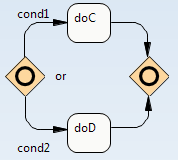
\includegraphics[width=0.3\textwidth]{images/mapping/or-gateway.png}} &  & \texttt{[...]}\\
	& & \texttt{Thread and\_branch1 = new Thread()\{}\\
	& & \texttt{\hspace{10pt}public void run()\{}\\
	& & \texttt{\hspace{20pt}if(cond1)\{}\\
	& & \texttt{\hspace{30pt}doC();}\\
	& & \texttt{\hspace{20pt}\}}\\
	& & \texttt{\hspace{10pt}\}}\\
	& & \texttt{\};}\\
	& & \texttt{Thread and\_branch2 = new Thread()\{}\\
	& & \texttt{\hspace{10pt}public void run()\{}\\
	& & \texttt{\hspace{20pt}if(cond2)\{}\\
	& \textbf{\textcolor{blue}{=}} & \texttt{\hspace{30pt}doB();}\\
	& & \texttt{\hspace{20pt}\}}\\
	& & \texttt{\hspace{10pt}\}}\\
	& & \texttt{\};}\\
	& & \texttt{and\_branch1.start();}\\
	& & \texttt{and\_branch2.start();}\\
	& & \texttt{try \{}\\
	& & \texttt{\hspace{10pt}and\_branch1.join();}\\
	& & \texttt{\hspace{10pt}and\_branch2.join();}\\
	& & \texttt{\} catch(InterruptedException) \{ \}}\\
	& & \texttt{[...]}\\
\end{tabularx}
\caption{Mapping : OR Gateway}%
\label{fig:mapping_OR}%
\end{figure}


\textbf{XOR\_Data-Gateway (Exclusive)}\\
Branches of an XOR\_Data are wrapped in an if-then-else block (see Figure \ref{fig:xorData}). Only one branch will actually be executed at runtime. \\

\begin{figure}[h]
\begin{tabularx}{\linewidth}{lcX}
	\multirow{9}{*}{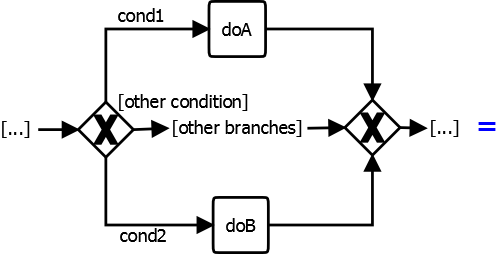
\includegraphics[width=0.3\textwidth]{images/mapping/xor-data.png}} &  & \texttt{[...]}\\
	& & \texttt{if(cond1)\{}\\
	& & \texttt{\hspace{10pt}doE();}\\
	& & \texttt{\} else \{}\\
	& \textbf{\textcolor{blue}{=}} & \texttt{\hspace{10pt}if(cond2)\{}\\
	& & \texttt{\hspace{20pt}doF();}\\
	& & \texttt{\hspace{10pt}\}}\\
	& & \texttt{\}}\\
	& & \texttt{[...]}\\
\end{tabularx}
\caption{Mapping : XOR\_Data Gateway}%
\label{fig:mapping_xorData}%
\end{figure}

\textbf{XOR\_Event-Gateway (Event Based)}\\
For XOR\_Event, a waiting loop will be started in a Thread, and an EventHandler (an extension to java.lang.Thread) instance for each branch will be created and started, according to the event's trigger of each branch. If an event handler recieve an event, the waiting thread will be stopped, and the process continues with the elements of the branch, and other branches will be skipped. The event handler will be added as an inner class to the bean, and they will have a constructor with a Thread toStop argument (among other arguments). \\
Figure \ref{fig:mapping_xorEvent} shows an example of the mapping.

\begin{figure}[h]
\begin{tabularx}{\linewidth}{lcX}
	\multirow{26}{*}{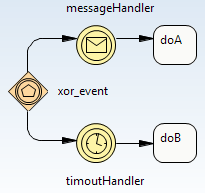
\includegraphics[width=0.3\textwidth]{images/mapping/xor-event.png}} &  & \texttt{[...]}\\
	& & \texttt{Thread xor\_event\_wait = new Thread()\{}\\
	& & \texttt{\hspace{10pt}public void run()\{}\\
	& & \texttt{\hspace{20pt}while(true)\{}\\
	& & \texttt{\hspace{30pt}try\{}\\
	& & \texttt{\hspace{40pt}Thread.sleep(100);}\\
	& & \texttt{\hspace{30pt}\} catch(InterruptedException e) \{ \}}\\
	& & \texttt{\hspace{20pt}\}}\\
	& & \texttt{\hspace{10pt}\}}\\
	& & \texttt{\};}\\
	& & \texttt{MessageHandler messageHandler = new MessageHandler(xor\_event\_wait);}\\
	& \textbf{\textcolor{blue}{=}} & \texttt{Timeout timeoutHandler = new TimeoutHandler(20000, xor\_event\_wait);}\\
	& & \texttt{xor\_event\_wait.start();}\\
	& & \texttt{messageHandler.start();}\\
	& & \texttt{timeoutHandler.start();}\\
	& & \texttt{try\{}\\
	& & \texttt{\hspace{10pt}xor\_event\_wait.join();}\\
	& & \texttt{\hspace{10pt}timeoutHandler.stop();}\\
	& & \texttt{\hspace{10pt}messageHandler.stop();}\\
	& & \texttt{\} catch(InterruptedException e) \{}\\
	& & \texttt{\hspace{10pt}if(messageHandler.hasBeenTriggered())\{}\\
	& & \texttt{\hspace{20pt}doA();}\\
	& & \texttt{\hspace{10pt}\}}\\
	& & \texttt{\hspace{10pt}if(timeoutHandler.hasBeenTriggered())\{}\\
	& & \texttt{\hspace{20pt}doB();}\\
	& & \texttt{\hspace{10pt}\}}\\
	& & \texttt{\}}\\
	& & \texttt{[...]}\\
\end{tabularx}
\caption{Mapping : XOR\_Event Gateway}%
\label{fig:mapping_xorEvent}%
\end{figure}

\textbf{Complex-Gateway}\\
A mapping concept for Complex Gateways has not been developed in the current Version. \\
\subsection{Loop Blocks}
Structured loop blocks are mapped as shown in Figure \ref{fig:mapping_loop}.
\begin{figure}[h]
\begin{tabularx}{\linewidth}{lcX}
	\multirow{8}{*}{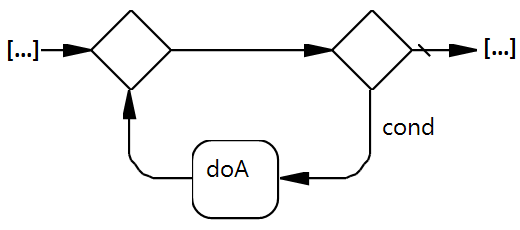
\includegraphics[width=0.3\textwidth]{images/mapping/loop_block.png}} &  &\\
	& & \texttt{[...]}\\
	& & \texttt{while(cond)\{}\\
	& & \texttt{\hspace{10pt}doA();}\\
	& \textbf{\textcolor{blue}{=}} & \texttt{\}}\\
	& & \texttt{doB();}\\
	& & \texttt{[...]}\\
	& & \\
\end{tabularx}
\caption{Mapping example: Loop Blocks }%
\label{fig:mapping_loop}%
\end{figure}

While the condition applies, the content branch will be repeated. 

\begin{figure}[h]
\begin{tabularx}{\linewidth}{lcX}
	\multirow{29}{*}{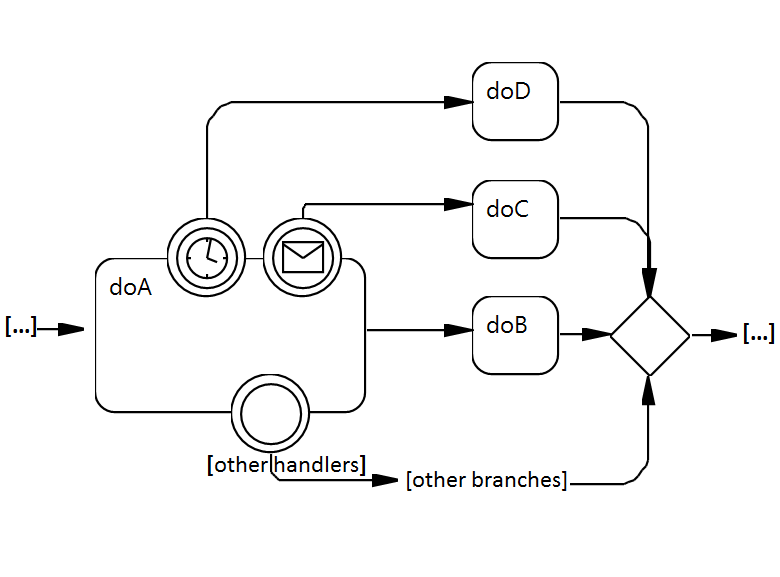
\includegraphics[width=0.4\textwidth]{images/mapping/event_handler.png}} &  & \texttt{Thread doA\_Thread = new Thread()\{}\\
	& & \texttt{\hspace{10pt}public void run()\{}\\
	& & \texttt{\hspace{20pt}doA();}\\
	& & \texttt{\hspace{10pt}\}}\\
	& & \texttt{\};}\\
	& & \texttt{MessageHandler messageHandler = new MessageHandler(doA\_Thread);}\\
	& & \texttt{TimeoutHandler timeoutHandler = new TimeoutHandler(20000, doA\_Thread);}\\
	& & \texttt{doA\_Thread.start();}\\
	& & \texttt{messageHandler.start();}\\
	& \textbf{\textcolor{blue}{=}} & \texttt{timeoutHandler.start();}\\
	& & \texttt{try\{}\\
	& & \texttt{\hspace{10pt}doA\_Thread.join();}\\
	& & \texttt{\hspace{10pt}timeoutHandler.stop();}\\
	& & \texttt{\hspace{10pt}messageHandler.stop();}\\
	& & \texttt{\} catch(InterruptedException e) \{}\\
	& & \texttt{\hspace{10pt}if(messageHandler.hasBeenTriggered()\{}\\
	& & \texttt{\hspace{20pt}doD();}\\
	& & \texttt{\hspace{10pt}\}}\\
	& & \texttt{\hspace{10pt}if(timeoutHandler.hasBeenTriggered()\{}\\
	& & \texttt{\hspace{20pt}doC();}\\
	& & \texttt{\hspace{10pt}\}}\\
	& & \texttt{\}}\\
	& & \texttt{if(!messageHandler.hasBeenTriggered())\{}\\
	& & \texttt{\hspace{10pt}if(!timeoutHandler.hasBeenTriggered())\{}\\
	& & \texttt{\hspace{20pt}doB();}\\
	& & \texttt{\hspace{10pt}\}}\\
	& & \texttt{\}}\\
\end{tabularx}
\caption{Mapping : Event Handler}%
\label{fig:mapping_eventhandler}%
\end{figure}

\subsection{Event Handler}
As we can see in Figure \ref{fig:mapping_eventhandler}, the mapping of an Event Handler attached to an activity is somewhat similar to the mapping of gateway event. Instead of the waiting thread, a thread calling the activity method will be created, and it will be stopped if the event handler is triggered.\\

\newpage
\section{Activites}
Now we will discuss the activities in details. Activities are divided into tasks and subprocess. As mentioned before, task will be wrapped in an activity method. This enables each task to have their own scope of properties. The properties of subprocesses however, should be shared with all activities contained in it. Therefore wrapping subprocesses in a method is not enough. Instead a subprocess will be wrapped in an inner class.
 
\subsection{Tasks}
Basically, a task will be mapped as follows:

\begin{figure}[h]
\centering%
\begin{tabularx}{\linewidth}{lcX}
	\multirow{8}{*}{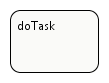
\includegraphics[width=0.25\textwidth]{images/mapping/task.png}} &  &\\
	& & \texttt{public void doTask()\{}\\
	& & \texttt{\hspace{10pt}[declaration of properties]}\\
	& \textbf{\textcolor{blue}{=}} & \texttt{\hspace{10pt}[start assignments]}\\
	& & \texttt{\hspace{10pt}[special mapping depending on task-type]}\\
	& & \texttt{\hspace{10pt}[end assignments]}\\
	& & \texttt{\}}\\
	& & \\
\end{tabularx}
\caption{Mapping example: Task}%
\label{fig:mapping_task}%
\end{figure}

The method will start by declaring java variables, derived from the task's properties(if any exists). After the declaration, start assignments will take place, followed by the task's actual mapping (if any, depending on the task type). Now let's take a closer look on how specific task types are being mapped.\\

\textbf{Script-task}\\
For Script-tasks, the script defined in the task's property will be directly added into the activity-method. This type of task is comparable to Wade's \textit{Code Activity}. For the transformation to agent beans, the given script should be a valid Java expression.\\\\

\textbf{Service-task}\\
A service task is mapped into an invocation of an Action defined by other Bean.\\

\begin{figure}[h]
\begin{tabularx}{\linewidth}{lcX}
	\multirow{5}{*}{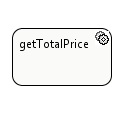
\includegraphics[width=0.25\textwidth]{images/mapping/service_task.png}} & & \texttt{ [...]}\\
	& & \texttt{Action [operation] = retrieveAction([interface].[operation]);}\\
	& \textbf{\textcolor{blue}{=}} & \texttt{Serializeable [] results = invokeAndWaitForResults([operation], new Serializeable[]\{[inputs]\}).getResults();}\\
  & & \texttt{[assign outputs from results]}\\
  & & \texttt{[...]}
\end{tabularx}
\caption{Mapping example: Service-task}%
\label{fig:service_task}%
\end{figure}
Figure \ref{fig:service_task} shows how a service task would be mapped. First, the action has to be found. Then the service will be invoked and the result will be assign to the outputs defined in the task's implementing Service.\\\\

\textbf{Send-task}\\
A Send task will be mapped into an invocation of the ICommunicationBean's send action (see Figure \ref{fig:send_task}). The group address, to which the message should be sent, and the message itself will be derived from the given MessageChannel in the task's properties. \\\\
 
\begin{figure}[h]
\begin{tabularx}{\linewidth}{lcX}
	\multirow{6}{*}{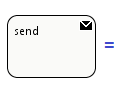
\includegraphics[width=0.25\textwidth]{images/mapping/sendTask.png}} & & \texttt{[...]}\\
	& & \texttt{Action sendAction = retrieveAction(ICommunicationBean.ACTION\_SEND);}\\
	& \textbf{\textcolor{blue}{=}} & \texttt{IGroupAddress groupAddress = CommunicationAddressFactory.createGroupAddress([address]);}\\
	& & \texttt{JiacMessage jiacMessage = new JiacMessage([payload]);}\\
	& & \texttt{invoke(sendAction, new Serializable[]\{jiacMessage, groupAddress\});}\\
 & & \texttt{[...]}
\end{tabularx}
\caption{Mapping example: Send-task}%
\label{fig:send_task}%
\end{figure}


\textbf{Recieve-task}\\
A Recieve-task will be mapped into a Java-Code that reads the memory and wait until the specified message defined by the given MessageChannel is found in the memory. \\

\begin{figure}[h]
\begin{tabularx}{\linewidth}{lcX}
	\multirow{6}{*}{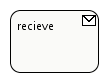
\includegraphics[width=0.25\textwidth]{images/mapping/recieveTask.png}} & & \texttt{[...]}\\
	& & \texttt{Action sendAction = retrieveAction(ICommunicationBean.ACTION\_SEND);}\\
	& \textbf{\textcolor{blue}{=}} & \texttt{IGroupAddress groupAddress = CommunicationAddressFactory.createGroupAddress([address]);}\\
	& & \texttt{JiacMessage jiacMessage = new JiacMessage([payload]);}\\
	& & \texttt{invoke(sendAction, new Serializable[]\{jiacMessage, groupAddress\});}\\
 & & \texttt{[...]}
\end{tabularx}
\caption{Mapping example: Send-task}%
\label{fig:recieve_task}%
\end{figure}


\textbf{Other-tasks (currently not mapped)}
There are still other task-types for which the mapping concept has not been developed yet. This includes:
\begin{enumerate}
	\item User-task
	\item Manual-task
	\item Call-task
	\iten BusinessRule-task
\end{enumerate}
\\\\

\subsection{Subprocess}
A subprocess will be mapped into an inner class of the containing Process or Subprocess. This way it's properties can be shared among all tasks contained in it. The inner subprocess will have the method \texttt{public void run()} containing the workflow (similar to the bean's workflow method). The following example shows the mapping of a subprocess:\\

\begin{figure}[h]
\centering
\begin{tabularx}{\linewidth}{lcX}
	\multirow{16}{*}{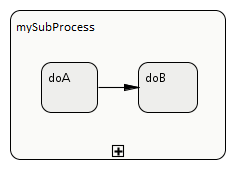
\includegraphics[width=0.35\textwidth]{images/mapping/subprocess.png}} &  &public void doProcess\{//workflow-method\\
	& & \texttt{\hspace{10pt}[...]}\\
	& & \texttt{\hspace{10pt}SubProcess subProcess = new SubProcess();}\\
	& & \texttt{\hspace{10pt}subProcess.run();}\\
	& & \texttt{\hspace{10pt}[...]}\\
	& & \texttt{\}}\\
	& & \texttt{[...]}\\
	& \textbf{\textcolor{blue}{=}} & \texttt{class SubProcess \{}\\
	& & \texttt{\hspace{10pt}[declaration of properties]}\\
	& & \texttt{\hspace{10pt}public void run()\{}\\
	& & \texttt{\hspace{20pt}doA();}\\
	& & \texttt{\hspace{20pt}doB();}\\
	& & \texttt{\hspace{10pt}\}}\\
	& & \texttt{\hspace{10pt}private void doA()\{ [...] \}}\\
	& & \texttt{\hspace{10pt}private void doB()\{ [...] \}}\\
	& & \texttt{\}}\\
\end{tabularx}
\caption{Mapping example : Subprocess}%
\label{fig:mapping_subprocess}%
\end{figure}

\subsection{Activity-Looping}
If an activity has a looping property in it's properties, then the mapped element will be wrapped in a while-block. This is analog to the mapping of a structured Loop Block but the loop exists in an activity method instead of the workflow method.


\textbf{Standard-Loop}\\\\

\textbf{Multi-Instance Loop}\\\\


\section{Events}

\subsection{Start-Events}

\textbf{Timer}\\
\\\\

\textbf{Message}\\
\\\\

\subsection{Intermediate-Events}
\textbf{Timer}\\
\\\\

\textbf{Message}\\
\\\\

\subsection{End-Events}


\section{Open Issues}